\documentclass[12pt letterpaper]{article}

\usepackage{fullpage}
\usepackage{graphicx}
\usepackage{amsmath}

\providecommand{\e}[1]{\ensuremath{\times 10^{#1}}}
\usepackage{gensymb}

\usepackage{float}


\title{Statistics In Counting Experiments}
\author{Johnny Minor \\ Partner: Kayla Mitchell}
\date{\today}

\begin{document}

\maketitle

%abstract should have a very brief overiew of the goals and main results of the experiment. 
\begin{abstract}
In this experiment we study the nature of long-lived radioactive sources and their emission. We made 100 counts of the cosmic and background radiation with a scintillator. We then placed a provided radioactive source in from of the scintillation detector and made 100 counts. We also used a Geiger detector to make 100 counts of the period between two successive counts. We created normalized freqeuncy histograms for each experiment and fit a Poisson distribution, Gaussian distribution, and a Gaussian distribution with a calculated standard deviation. We found that in general for low counts the Poisson distribution fits well. For high counts neither Poisson or Gaussian fit our experimental data very well, but the Gaussian fit slightly better. 
\end{abstract}

\newpage

\section*{Description of Experiment}

In this experiment we studied randomly occurring events. The event we studied was the emission from a long-lived radioactive source. In order to study this we used a scintillation counter. The active element within it is a 1 x 1 inch NaI crystal. 

\begin{figure}[H]
  \caption{Schematic of a scintillation counter.}
  \centering
    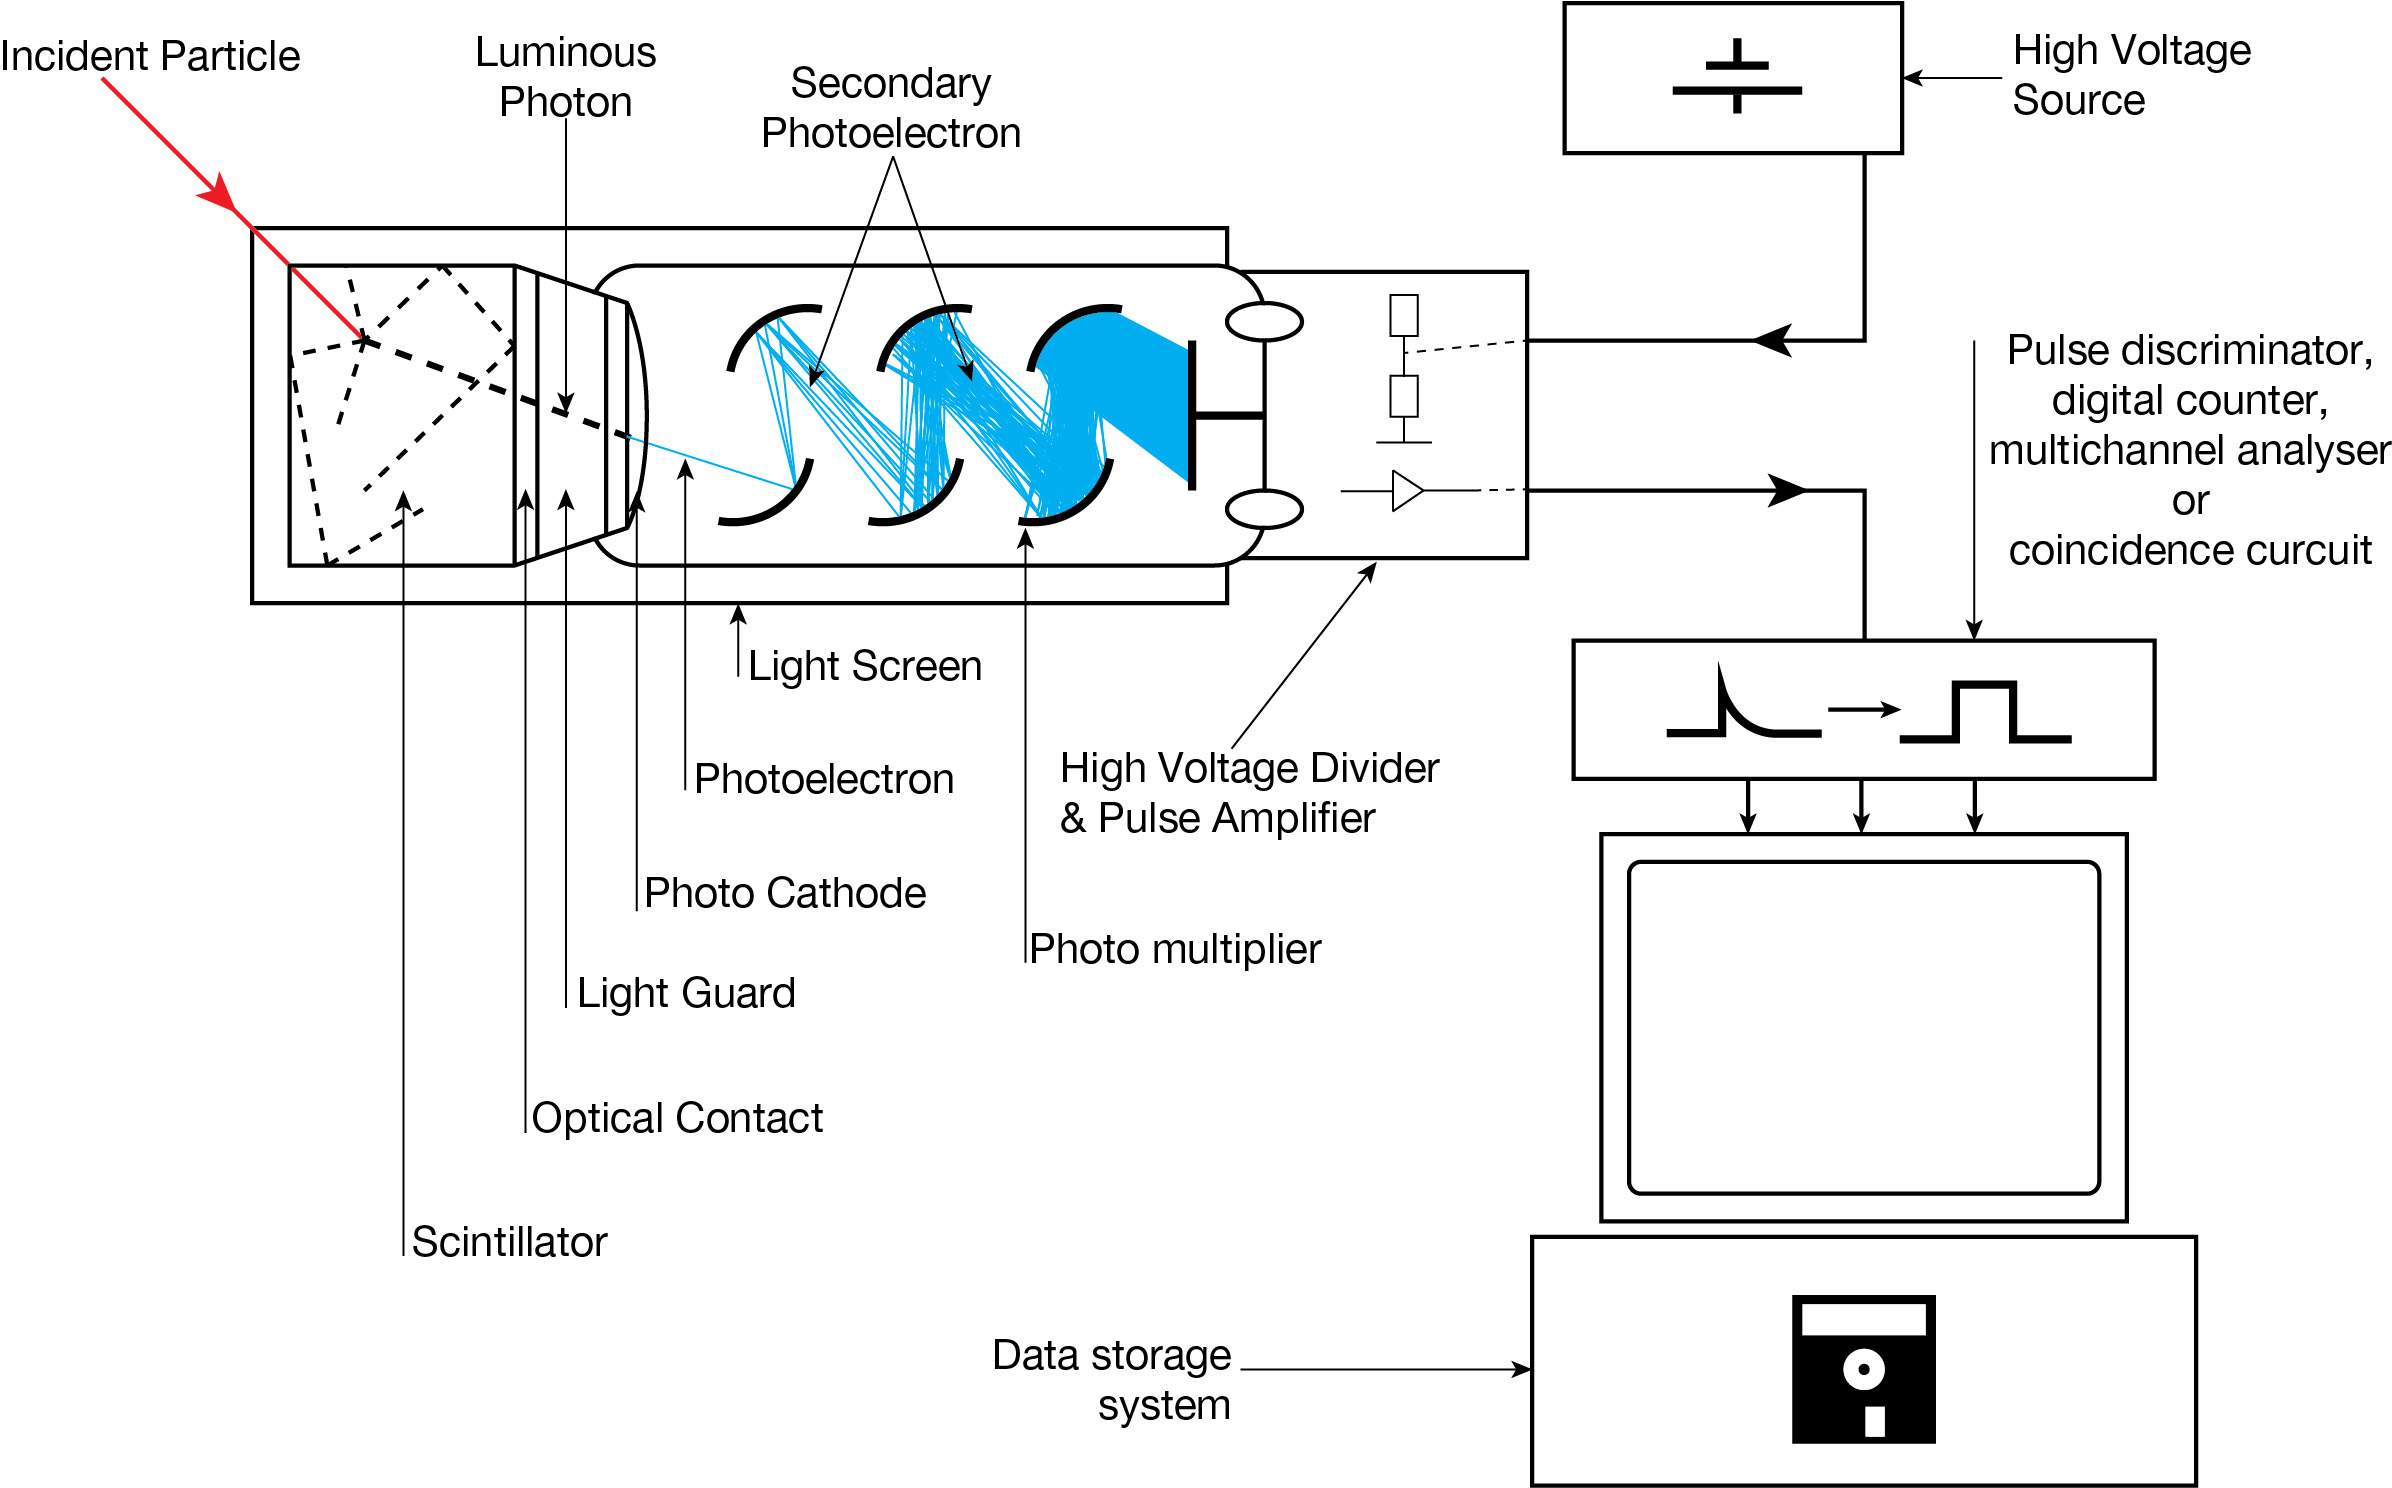
\includegraphics[width=.5\textwidth]{scintillation.jpg}
    \label{fig:scintillator}
\end{figure}

For the small average counts we set the the voltage to be 1500 volts to get a frequency count with an average of around 2. In the second part we used the provided radioactive source and increased the voltage to 1900 volts to get an average frequency count of around 100. We recorded this data into Origin. After facing unrivaled technical difficulties using Origin for data analysis was forfeited in favor of different software. 

In our third experiment we used a Geiger detector and a time interval counter set to 'period' mode. With this setting it counts the time passed between two detections. A cosmic ray should be detected about once a second using this method. We collected 100 points of data for this method. Once again logging our data in Microsoft Excel. 

\begin{figure}[H]
  \caption{A schematic of a Geiger counter.}
  \centering
    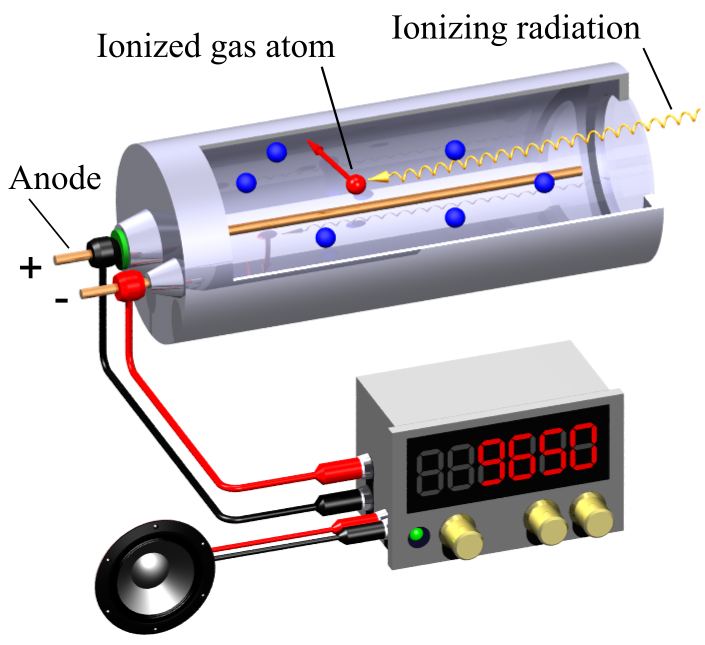
\includegraphics[width=.5\textwidth]{geiger.png}
    \label{fig:geiger}
\end{figure}


In our fourth experiment we didn't have a divide-by-n circuit so we just summed pairs of intervals between subsequent pulses, as instructed in the handout. To get a new distribution. 

In order to create our plots it was important to choose a bin width that allowed us to see a pattern. Too small a bin width would just make a frequency histogram with either 1 or 0(at least for the higher counts) because the probability of getting the same number between zero and 250 is small. Further, if we chose a bin width too large we wouldn't be able to see any distinguishing features because everything would just be jumbled together. 


When we fit our data we first had to normalize our data. In order to do this we took our frequency and then divided by the total number of counts. In all cases we had 100 counts. This leads to the data summing to 1. Furthermore, as we found, the value for Poisson and Gaussian had to be multiplied by the bin width. This makes sense because we need our probability distribution to sum to one in order to make sense. Furthermore, it makes good sense because if we only had one point for an interval that was greater than one (or less than one). 


\section*{Data and Analysis}

In order to see how good data is qualitatively we plotted either a Poisson distribution or a Gaussian distribution on top of our histogram. The Poisson distribution is 
\begin{equation}
\label{eq:poisson}
P(x) = \frac{\mu^x e^{- \mu}}{x!}
\end{equation}

where $\mu$ is the average of the data set, and $x$ is the bin. As we have learned Poisson is a better distribution when our values are small, but greater than 0. So, we would expect it to be a better fit in the first experiment where the average is around 2, but a poor fit when the average count is around 100. When the average count is higher we would expect a Gaussian distribution to be a much better fit. 

A Gaussian distribution is used when we have many independent events that occur. The equation for this distribution is 
\begin{equation}
P(x) = \frac{1}{\sigma\sqrt{2\pi} } \; e^{ -\frac{(x-\mu)^2}{2\sigma^2} }
\end{equation}

where $\sigma$ is the variance, $\mu$ is the average, and $x$ is the bin. We know that the Gaussian distribution should be a better fit for numerous independent events. 

\subsection*{Small Average Number of Counts}

\begin{figure}[H]
  \caption{A graph of our experimental data with corresponding Poisson distribution.}
  \centering
    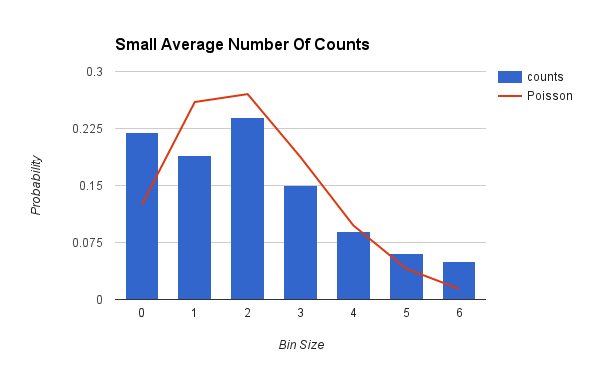
\includegraphics[width=.75\textwidth]{section1_1_1.png}
    \label{fig:section1.1.1}
\end{figure}

We can see in \ref{fig:section1.1.1} that our data follows the calculated Poisson distribution fairly well. We found the average to be 2.08 for our experiment with a standard deviation of 1.72. Our standard deviation is relatively close to the expected value with the Poisson distribution of 1.44. 


\subsection*{Large Average Number of Counts}

\begin{figure}[H]
  \caption{A graph of our experimental data with corresponding Poisson distribution.}
  \centering
    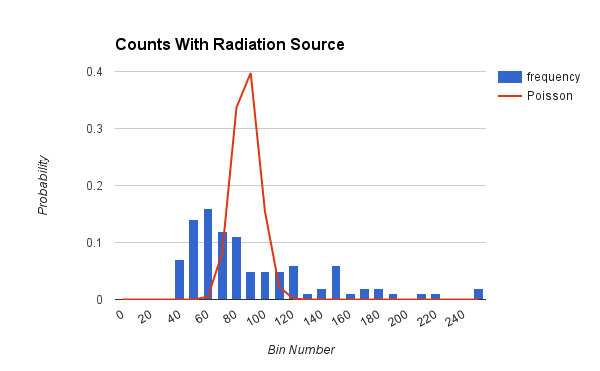
\includegraphics[width=.75\textwidth]{section1_1_2_poisson.png}
    \label{fig:section1.1.2poisson}
\end{figure}

\begin{figure}[H]
  \caption{A graph of our experimental data with corresponding Gaussian distribution.}
  \centering
    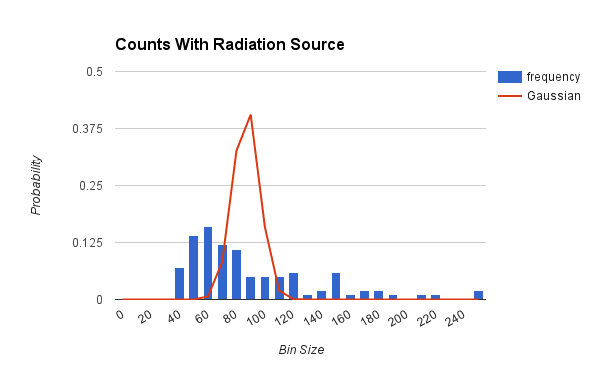
\includegraphics[width=.75\textwidth]{section1_1_2_gaussian.png}
    \label{fig:section1.1.2gaussian}
\end{figure}

Here our data clearly does not fit very well with either a calculated Poisson or Gaussian. In this Gaussian calculation we used the mean of 86.88 and, as instructed, used the standard deviation as the square root of the mean. Which we calculated to be 9.32. It is also important to note that although the two graphs looks identical they are in fact not! The values are very slightly different. We believe this is due to the very poor fit of the Gaussian distribution because of the artificially poor standard deviation. When we calculate the true standard deviation we find it to be 47.93. This is much higher than the 9.32 and it clearly shows when we compare figure \ref{fig:section1.1.2gaussian} and \ref{fig:section1.1.2gaussianstddev}. 

\begin{figure}[H]
  \caption{A graph of our experimental data with corresponding Gaussian distribution with calculated standard deviation.}
  \centering
    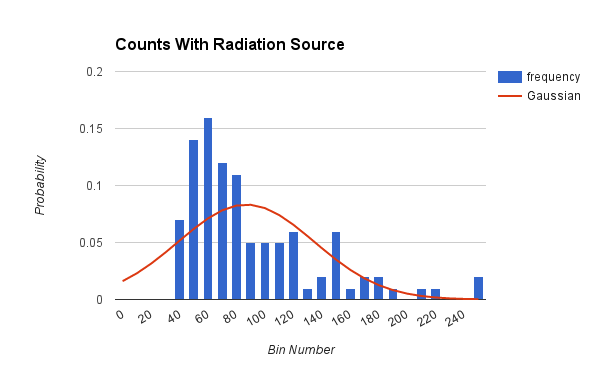
\includegraphics[width=.75\textwidth]{section1_1_2_gaussian_std_dev.png}
    \label{fig:section1.1.2gaussianstddev}
\end{figure}

Although this fits better than what we found in figure \ref{fig:section1.1.2gaussian}, but it still does not inspire confidence. Clearly our data has too high a frequency from around 40 to 90. We believe that this could be due to selection bias of numbers, or simply that we don't have a higher enough number of counts. Perhaps our data would better resemble a Gaussian distribution if we had 1000 counts. 

\subsection*{Distribution of Time Intervals Between Successive Counts}

\begin{figure}[H]
  \caption{A graph of our experimental data with Poisson distribution.}
  \centering
    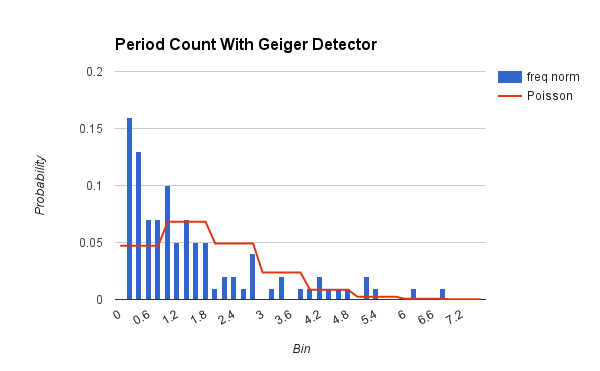
\includegraphics[width=.75\textwidth]{section1_2_1_poisson.png}
    \label{fig:section1.2.1poisson}
\end{figure}

In this experiment we plotted a Poisson distribution using our calculated mean of 1.45. The Poisson distribution doesn't seem to fit very well because our data seems to be too skewed to the left i.e. towards zero. 

\begin{figure}[H]
  \caption{A graph of our experimental data with corresponding Gaussian distribution with calculated standard deviation.}
  \centering
    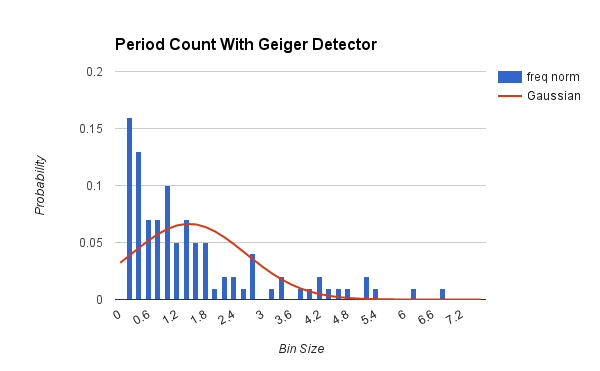
\includegraphics[width=.75\textwidth]{section1_2_1_gaussian.png}
    \label{fig:section1.2.1gaussian}
\end{figure}

\begin{figure}[H]
  \caption{A graph of our experimental data with corresponding Gaussian distribution with calculated standard deviation.}
  \centering
    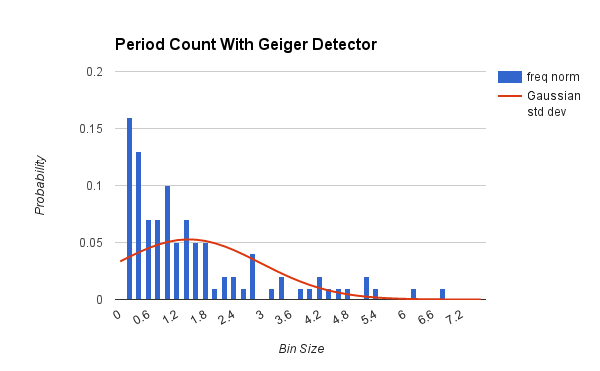
\includegraphics[width=.75\textwidth]{section1_2_1_gaussian_std_dev.png}
    \label{fig:section1.2.1gaussianstddev}
\end{figure}

If we fit a Gaussian and also a Gaussian with our calculated standard deviation of 1.51 then we find that it still doesn't fit very well. This could be due to poor data that we collected. Perhaps the instrumentation was not that accurate, or we received more radiation than we had expected. Thus resulting in very short times between successive counts. We could also consider taking more data to get a better fit. 

\subsection*{Distribution of Time Intervals Between Every Other Count}

\begin{figure}[H]
  \caption{A graph of our experimental data with corresponding Gaussian distribution with calculated standard deviation.}
  \centering
    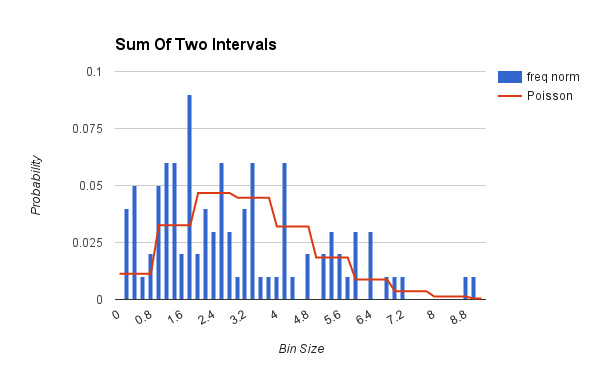
\includegraphics[width=.75\textwidth]{section1_2_2_poisson.png}
    \label{fig:section1.2.2poisson}
\end{figure}

As stated earlier we didn't have a divide-by-n circuit so we just summed two intervals together. This lead to these graphs. Which also don't fit very well.

\begin{figure}[H]
  \caption{A graph of our experimental data with corresponding Gaussian distribution with calculated standard deviation.}
  \centering
    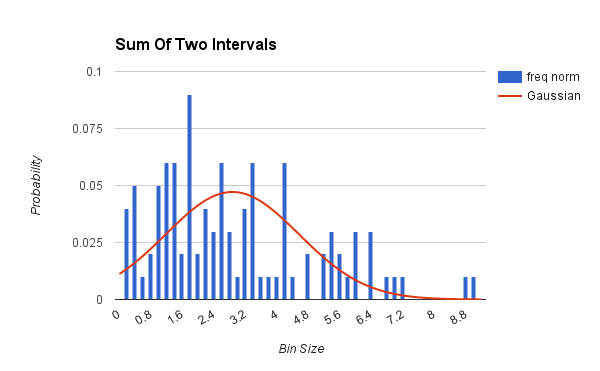
\includegraphics[width=.75\textwidth]{section1_2_2_gaussian.png}
    \label{fig:section1.2.2gaussian}
\end{figure}

In figure \ref{fig:section1.2.2poisson} we plotted a Poisson distribution with a calculated average of 2.89. This clearly does not fit well whatsoever. 

\begin{figure}[H]
  \caption{A graph of our experimental data with corresponding Gaussian distribution with calculated standard deviation.}
  \centering
    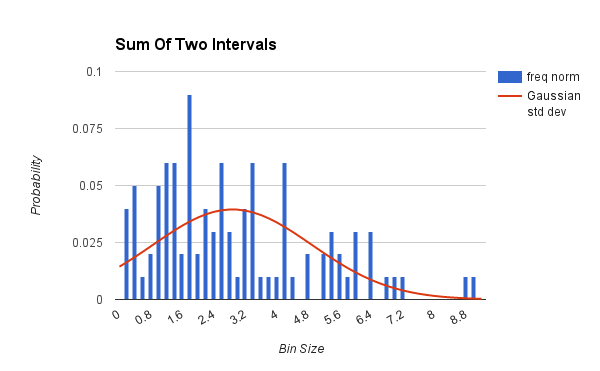
\includegraphics[width=.75\textwidth]{section1_2_2_gaussian_std_dev.png}
    \label{fig:section1.2.2gaussianstddev}
\end{figure}

When we calculate the standard deviation we get 2.02. This is somewhat close to the square root of the average of 1.69. However, this still doesn't lead to a good fit of our data with either of the Gaussian distributions. It seems that there are just some bins that accrue a high probability that throws everything off. Clearly the data is poor and we could perhaps remedy this with a great amount of data. 


\section*{Results and Conclusions}

In this experiment we found that the Poisson distribution does seem to fit well with our experimental data when the numbers are small. When the numbers are large the Poisson distribution is a poor fit, and so is the Gaussian distribution when using a the square root of the mean as the standard deviation. When we calculate the actual standard deviation then we get a much better fit of the data with a Gaussian distribution. However, it still does not fit that well, but it's definitely better. 

In our experiment measuring the time intervals between counts we found that none of the distributions fit very well in both cases. The Poisson distribution seems to fit poorly, but somewhat close to the experimental data. The Gaussian doesn't fit whatsoever. 

\subsection*{Additional Questions}

a. Okay, we won't allow the tube to operate in the continuous discharge region because that would destroy the tube! I don't think the Geiger detector we were using had an option to vary the voltage of the detector. We know that the Geiger detector works with a Geiger-M\"uller tube filled with inert gas that when the gas interacts with the ionizing radiation it creates a pulse that we can then detect. 

\medskip
\noindent b. The Geiger counter is best at detecting ionizing radiation such as alpha particles, beta particles, and gamma rays. This is because of the Geiger-M\"uller tube that is central to the Geiger counter has an inert gas inside it that is very sensitive to the impinging radiation. The ionization of the gas paired with the Townsend avalanche phenomena leads to having a good detector. 

\medskip
\noindent c. No, the Geiger detector cannot be used to measure the energy of incident radiation. This is because the radiation ionizes the gas and then the gas sends a pulse to to the apparatus. So no energy is measured directly. As Melissino's states: "The disadvantages of the Geiger counter are the loss of all information on the ionizing power of the charged particle that traversed the counter..."  

\medskip 
\noindent d. We could measure the dead time by using a pulse interval discriminator that triggers the oscilloscope only when the counter is in a fully recovered state. (from J L Putman and E H Cooke-Yarborough). We don't think you would need to take into account the dead time in this experiment because we don't need that level of resolution since we are measuring in seconds. Furthermore, we are counting the period between two successive counts. 

\end{document}